\documentclass[11pt, oneside]{article}
\usepackage[letterpaper, margin=2cm]{geometry}
\usepackage{MATH566}
%\usepackage{sagetex}

\begin{document}
\noindent \textbf{\Large{Caleb Logemann \\
MATH 566 Discrete Optimization\\
Final
}}

%\lstinputlisting[language=Sage]{03_2.sage}
\begin{enumerate}
  \item % #1
Emperor has decided to build Death Star II. He needs  money to pay for it. He sent you to collect taxes from
several planets. Here are the coordinates of the planets assigned to you. You are starting at Corusant (0,0) and want to
return there. The time of travel between the planets corresponds to their Euclidean distance.
You have to visit all planets. Minimize the travel time.
\begin{verbatim}
X = [  [0,0], [9,0], [1,1], [8,1], [0,2], [9,2], [4,3], [5,3], \
[0,4], [1,4], [2,4], [3,4], [6,4], [7,4], [8,4], [9,4], \
[0,5], [1,5], [3,5], [2,5], [6,5], [7,5], [8,5], [9,5], \
[4,6], [5,6], [0,7], [9,7], [1,8], [8,8], [0,9], [9,9] ];
\end{verbatim}
  \item % #2
    You are leading a group $4$ of imperial fighters that are protecting an
    imperial shuttle transporting secret plans to Death Star II. 
    You were ambushed by $3$ rebel ships. You must protect the secret plans! Do not repeat the same mistake that happened with Death Star.

    Choose one fighter from your group to accompany the transport shuttle cover their retreat by fighting the rebel ship.
    The remaining three ships will each try to fight one rebel ship. You need to fight against each of the rebel ships to prevent
    pursuit of the transport shuttle and you do not want to leave the transport ship unguarded.

    For the remaining 3 ships that fight the rebel ships, maximize the total damage (sum of damages) caused to the rebel ships.
    For every pair of imperial and rebel ship, the damage caused by imperial ships to rebel ships is described in the following table.
    \begin{center}
      \begin{tabular}{c|ccccc}
              & $r_1$ & $r_2$ & $r_3$ \\ \hline
        $i_1$ &    3  &     2 &     3 \\
        $i_2$ &    2  &     3 &     1 \\
        $i_3$ &    4  &     2 &     2 \\
        $i_4$ &    1  &     5 &     1 \\
      \end{tabular}
    \end{center}
  \item % #3
    Darth Vader forgot his lightsaber.
    Bring it to him as fast as you can so the Emperor can watch a lightsaber
    fight between Darth Vader and Luke Skywalker.
    You have only a small ship and hence you need refueling.
    Here is a map of the space.
    Every planet has a number that corresponds to the time needed for refueling 
    and every connection has a travel time associated to it. 

    \begin{center}
      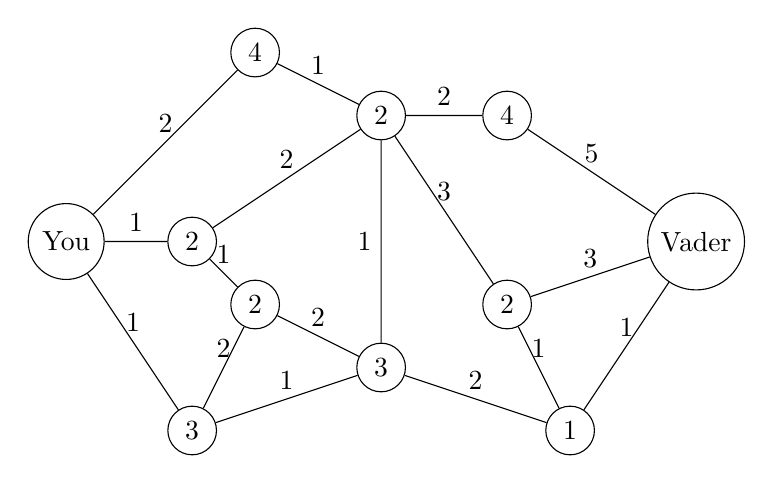
\begin{tikzpicture}[scale=0.8]
        \draw (0,0) node[circle,draw](y){You};
        \draw (10,0) node[circle,draw](v){Vader};
        \draw (2,-3) node[circle,draw](p1){3};
        \draw (3,3) node[circle,draw](p2){4};
        \draw (2,0) node[circle,draw](p3){2};
        \draw (5,-2) node[circle,draw](p4){3};
        \draw (5,2) node[circle,draw](p5){2};
        \draw (3,-1) node[circle,draw](p6){2};
        \draw (7,2) node[circle,draw](p7){4};
        \draw (7,-1) node[circle,draw](p8){2};
        \draw (8,-3) node[circle,draw](p9){1};
        \draw
          (y) -- node[above]{1} (p1)
          (y) -- node[above]{2} (p2)
          (y) -- node[above]{1} (p3)
          (p1) -- node[above]{1} (p4)
          (p1) -- node[above]{2} (p6)
          (p3) -- node[above]{1} (p6)
          (p3) -- node[above]{2} (p5)
          (p2) -- node[above]{1} (p5)
          (p5) -- node[above]{2} (p7)
          (p5) -- node[above]{3} (p8)
          (p5) -- node[left]{1} (p4)
          (p4) -- node[above]{2} (p6)
          (p4) -- node[above]{2} (p9)
          (p8) -- node[above]{1} (p9)
          (p8) -- node[above]{3} (v)
          (p9) -- node[above]{1} (v)
          (p7) -- node[above]{5} (v)
        ; 
      \end{tikzpicture}
    \end{center}

  \item % #4
    The Emperor, as any other good emperor, knows that it is best if his enemies
    are fighting among each other.
    Here is a map of Emperor's enemies and how much does it cost for each pair
    to start fighting each other.
    Find for the Emperor which pairs to trick into fighting each other such that
    every enemy is in exactly one fight.
    Provide also a certificate verifying the optimality of your solution.\\

    \emph{Provide optimal solution and certificate of optimality.}
    \begin{center}
      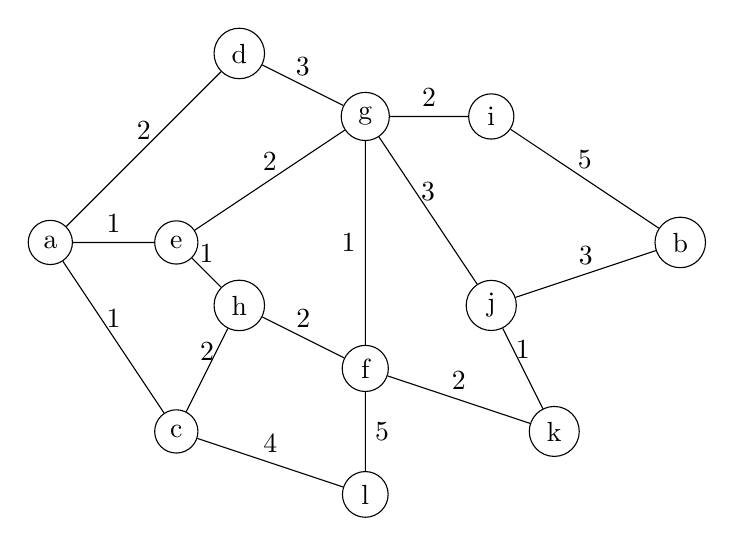
\begin{tikzpicture}[scale=0.8]
        \draw (0,0) node[circle,draw](y){a};
        \draw (10,0) node[circle,draw](v){b};
        \draw (2,-3) node[circle,draw](p1){c};
        \draw (3,3) node[circle,draw](p2){d};
        \draw (2,0) node[circle,draw](p3){e};
        \draw (5,-2) node[circle,draw](p4){f};
        \draw (5,2) node[circle,draw](p5){g};
        \draw (3,-1) node[circle,draw](p6){h};
        \draw (7,2) node[circle,draw](p7){i};
        \draw (7,-1) node[circle,draw](p8){j};
        \draw (8,-3) node[circle,draw](p9){k};
        \draw (5,-4) node[circle,draw](p10){l};
        \draw
          (y) -- node[above]{1} (p1)
          (y) -- node[above]{2} (p2)
          (y) -- node[above]{1} (p3)
          (p1) -- node[above]{2} (p6)
          (p3) -- node[above]{1} (p6)
          (p3) -- node[above]{2} (p5)
          (p2) -- node[above]{3} (p5)
          (p5) -- node[above]{2} (p7)
          (p5) -- node[above]{3} (p8)
          (p5) -- node[left]{1} (p4)
          (p4) -- node[above]{2} (p6)
          (p4) -- node[above]{2} (p9)
          (p8) -- node[above]{1} (p9)
          (p8) -- node[above]{3} (v)
          (p7) -- node[above]{5} (v)
          (p4) -- node[right]{5} (p10)
          (p1) -- node[above]{4} (p10)
        ; 
      \end{tikzpicture}
    \end{center}
\end{enumerate}
\end{document}
